Matematický model, ktorý opisuje biochemický reaktor je nelineárny model. To znamená, že odozva systému je rôzna pre rovnakú veľkosť skokovej zmeny pri rôznych začiatočných podmienkach. Túto nelinearitu si možno všimnúť na Obr. \ref{fig:1}. Ten opisuje časový priebeh koncentrácie Monod modelu pri viacerých skokových zmenách v rýchlosti riedenia $D = $ (0.2, 0.3, 0.4 a 0.5\unitfrac{1}{\hour}) so začiatočnými podmienkami $p_0 = s_0 = $ 0 \unitfrac{g}{L}, $x_0 = $ 10 \unitfrac{g}{L}. Parametre modelu boli nastavené ako to je uvedené v Tabuľke \ref{tab: 3}. Ďalej si môžeme všimnúť prudký nárast koncentrácie produktu na počiatku, ktorý bol spôsobený nadbytkom biomasy v systéme. Po ustálení dynamika produktu pripomína systém 1. rádu. Na druhej strane v dynamike tvorby biomasy sa prejavuje nestabilná nula (menšie podkmity), ktoré sú spôsobené v dôsledku zvýšenia prietoku látky cez reaktor. Keďže pritečie viac substrátu, čím sa zvýši jeho koncentrácia, koncentrácia biomasy naopak klesne, keďže odtečie viac suspenzie. Následne zvýšená koncentrácia substrátu podporí rast biomasy a tým sa aj koncentrácia biomasy začne zvyšovať. V dynamike substrátu sa zasa prejavuje stabilná nula, ktorá opäť súvisí s väčším prítokom čerstvého média a pomalšou spotrebou substrátu na tvorbu biomasy a produktu.

\begin{figure}
	\centering
	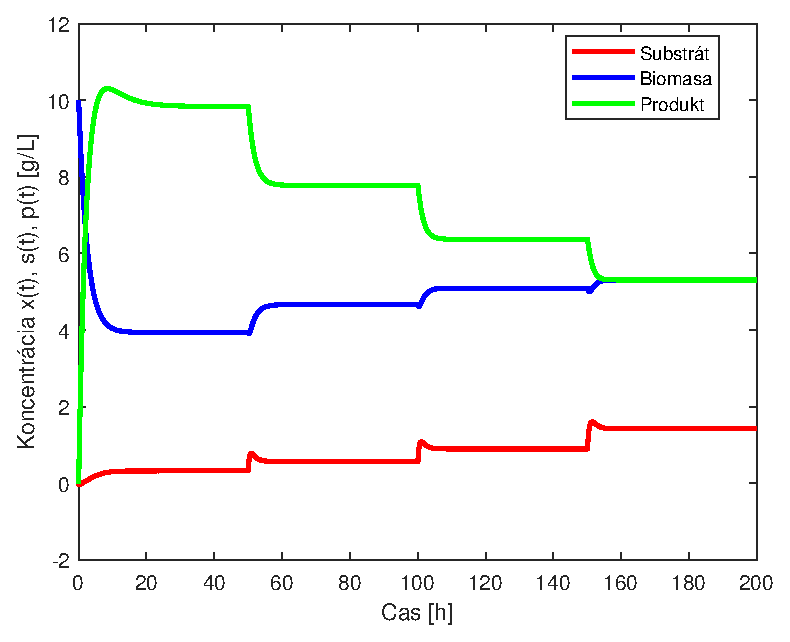
\includegraphics[width=.7\linewidth]{images/step_change}
	\caption[]{Časový priebeh koncentrácie substrátu, biomasy a produktu pri viacnásobnej skokovej zmene rýchlosti riedenia $D$ pri začiatočných podmienkach $p_0 = s_0 = $ 0, $x_0 = $ 10 \unitfrac{g}{L}.}
	\label{fig:1}
\end{figure}

Režim fungovania biochemického reaktora má významný vplyv na dynamiku celého systému a pri určitých podmienkach Monod model a model s inhibíciou môžu vykazovať rovnaké správanie, presne ako je tomu na Obr. \ref{fig:1}. Avšak, pri nesprávne zvolených pracovných podmienkach, či už počiatočných podmienkach systému, koncentrácie čerstvého substrátu alebo rýchlosti riedenia, model s inhibíciou bude vykazovať diametrálne odlišné správanie od Monod modelu, ako to je zobrazené na Obr. \ref{fig:3}. Na nich môžeme vidieť časové priebehy koncentrácie substrátu, biomasy a produktu pri rýchlosti riedenia $D = $ 0.4\unitfrac{1}{\hour} Monod modelu (Obr. \ref{fig:3}a) a modelu s inhibíciou (Obr. \ref{fig:3}b). Nastavenie parametrov modelov bolo ako je uvedené v Tabuľke \ref{tab: 3} a začiatočné podmienky boli $p_0 = s_0 = $ 0\unitfrac{g}{L}, $x_0 = $ 10\unitfrac{g}{L}. Ako môžeme vidieť, zatiaľ čo Monod model sa dostal do nenulového ustáleného stavu, model s inhibíciou klesol s koncentráciou biomasy a produktu na nulu, zatiaľ čo koncentrácia substrátu stúpla na hodnotu 20\unitfrac{g}{L}. Tento stav, kedy reaktorom preteká čistý substrát sa nazýva stav ,,vymytia`` alebo ,,výplach`` a prevádzka reaktora je nenávratne narušená.

\begin{figure}
	\begin{subfigure}{.5\textwidth}
		\centering
		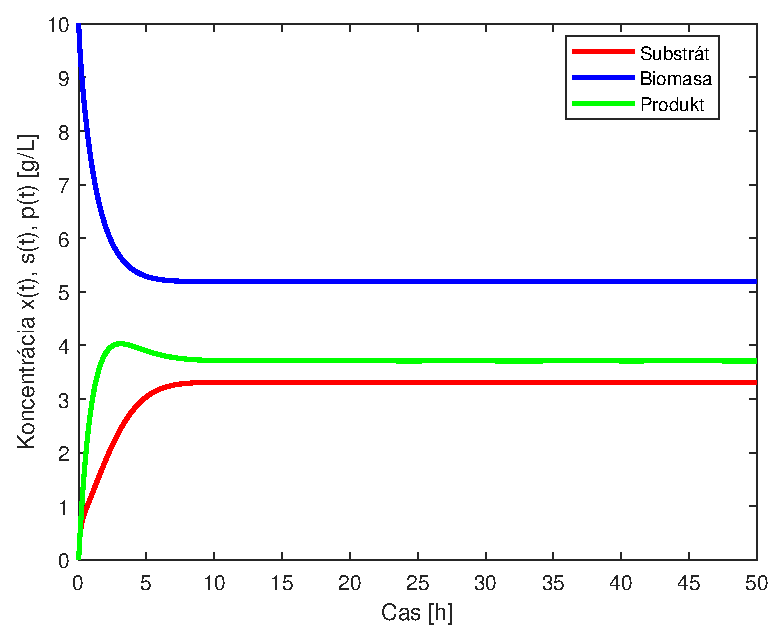
\includegraphics[width=1\linewidth]{images/dyn_Monod}
		\caption[]{Monod model}
	\end{subfigure}
	\begin{subfigure}{.5\textwidth}
		\centering
		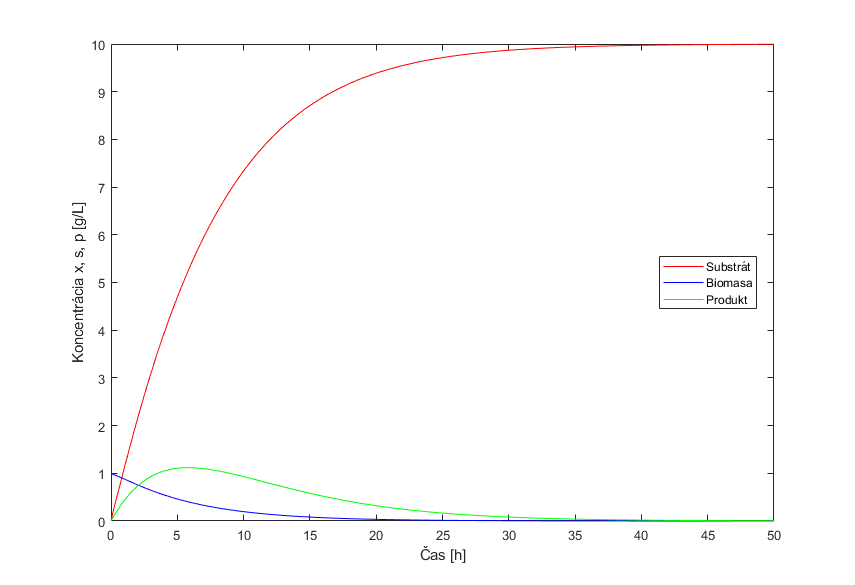
\includegraphics[width=1\linewidth]{images/dyn_inhb}
		\caption[]{Model s inhibíciou}
	\end{subfigure}
	\caption{Porovnanie dynamiky modelov pri rovnakých pracovných podmienkach.}
	\label{fig:3}
\end{figure}
